\chapter{Einleitung}
\label{cha:Einleitung}

\section{Motivation}
Für Enterprise-Resource-Planning(ERP)-Softwarelösungen ist es wichtig möglichst auf die Wünsche des Kunden einzugehen. Dies beinhaltet auch die Anpassung an bereits existierende Konkurrenzlösungen. 
Um hier nicht für jeden Drittanbieter eine eigene Schnittstelle implementieren zu müssen, versucht man, dies über eine Standardlösung, die international anerkannt ist, abzubilden. Hier hat sich speziell die eXtensible Markup Language (XML) etabliert. Die genannten Schnittstellen müssen stetig adaptiert und angepasst werden. 

Dies führt zu einem großen Entwicklungsaufwand, was die Validierung der einzelnen Daten bei der Kommunikation mit dem Fremdsystem betrifft. 
Im Vordergrund steht die Überprüfung der Datentypen der einzelnen Felder. Weiter sollen Pflicht- und Informationsfelder validiert, aber auch einfache Geschäftsregeln sollen kontrolliert werden können. 
Die Geschäftsregeln können dabei frei zwischen den Systemen definiert werden. Ein mögliches Beispiel wäre die Definition von Werten, die als Attribut von einzelnen XML-Elementen gesetzt werden. Aufgrund dieser Ausprägung müssen verschiedene andere Elemente mitgeliefert werden. Fehlen solche Abhängigkeiten, ist die XML-Datei ungültig und soll nicht importiert werden.

Die Validierung der kommunizierten Dateien erfolgt daher auf beiden Seiten der Schnittstellen. Mit einer automatisierten Variante, kann nun bereits vor der Inbetriebnahme der Schnittstelle beim Kunden, ein Fremdsystem ihre Kommunikation mit der ERP-Software überprüfen. 

Für die Validierung soll nun ein System entwickelt werden, dass am Besten standardisiert und international anerkannt ist.
Dabei liegt besonderer Aspekt auf Performance, Wartbarkeit und nötige Hilfsmittel die zur Validierung benötigt werden.


\section{Zielsetzung}
Das Ziel dieser Arbeit ist die Auswahl einer Technologie zur Validierung, die Beschreibung der notwendigen Schritte, um aus der definierten Schnittstelle eine Validierung-Datei zu erstellen. Die praktische Teil dieser Arbeit wurde dabei für die Firma \BMD erstellt. Die Definition der Schnittstellen erfolgt bei BMD über eine Auswahl von Felder, die über die Werte in einer Tabelle einer relationalen Datenbank gespeichert werden. 

Zum Beweis wird ein Prototyp erstellt, dessen Aus\-gabe eine Datei zur Validierung von XML-\-Dateien ist. Diese XML-Dateien dienen zum Austausch von Stamm-\- und Bewegungsdateien mit einem Fremd\-system. 
Die definierten Schnittstellen zu den Fremdsystemen variieren dabei sehr stark.

\begin{figure}
    \centering
    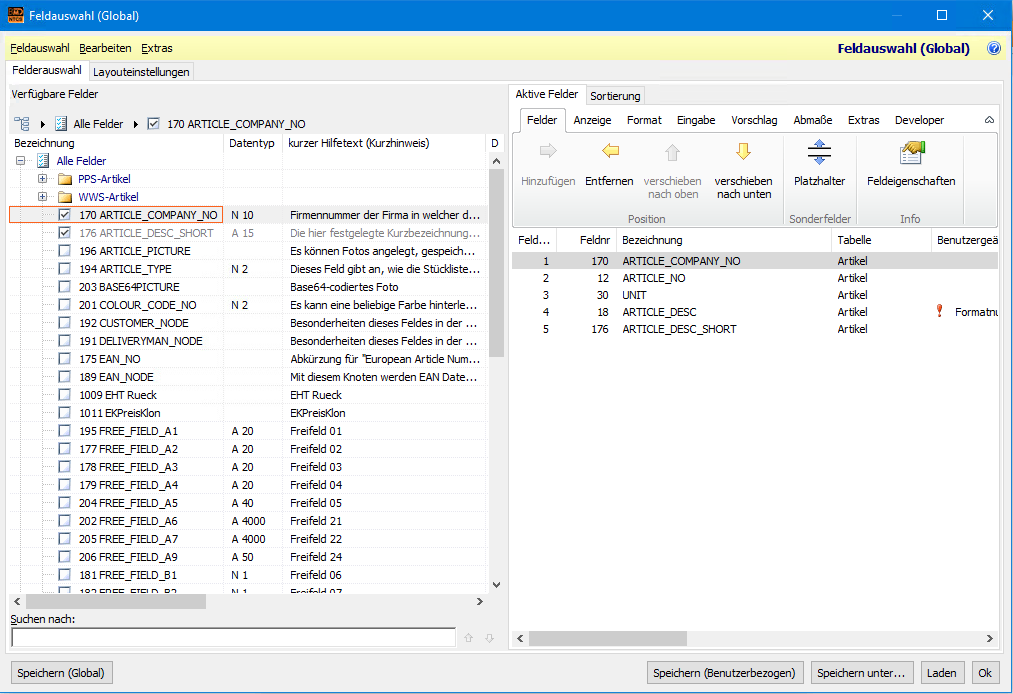
\includegraphics[width=.95\textwidth]{images/Feldauswahl.png}
    \caption{Definition Schnittstelle in BMD}
    \label{fig:Feldauswahl}
\end{figure}

Als Basis der Überprüfung dient deswegen eine Auswahl von 
verschiedenen Feldern, wie in Abbildung \ref{fig:Feldauswahl} dargestellt. 
Diese Felder repräsentieren jeweils eine Spalte einer relationalen Datenbank. 
Jede Auswahl ist wiederum in einer Tabelle gespeichert. 
Es müssen sowohl Oracle und Microsoft SQL Server unterstützt werden, da auch das ERP-System beide Datenbank-Systeme unterstützt. 
Konkret soll diese Software in das Modul der Produktionsplanungs- und Steuerungssystem (PPS) vom \BMD integriert werden. 
Dies bedeutet, dass der Prototyp keine eigen\-ständige Software sein soll oder muss. 
Den Fremdsystemen werden nur die Schemadateien zur Verfügung gestellt.

